The result of various SDN techniques which are used in HPC is presented here

\subsection{Evaluation of flow classification techniques}

In this section, I investigate how alternative flow-identification schemes affect the SDN routing algorithm across a suite of applications executed on two network topologies: a full-bisection fat-tree and a 3-to-1 tapered fat-tree. Application-level communication time serves as the primary performance metric. Throughout the experiments, I hold the routing policy constant at SDN-optimal and employ User-phase identification mechanism, systematically varying only the flow-identification technique.

\subsubsection{Performance Under full bisection fat-tree}
\begin{figure}[h]
  \centering
  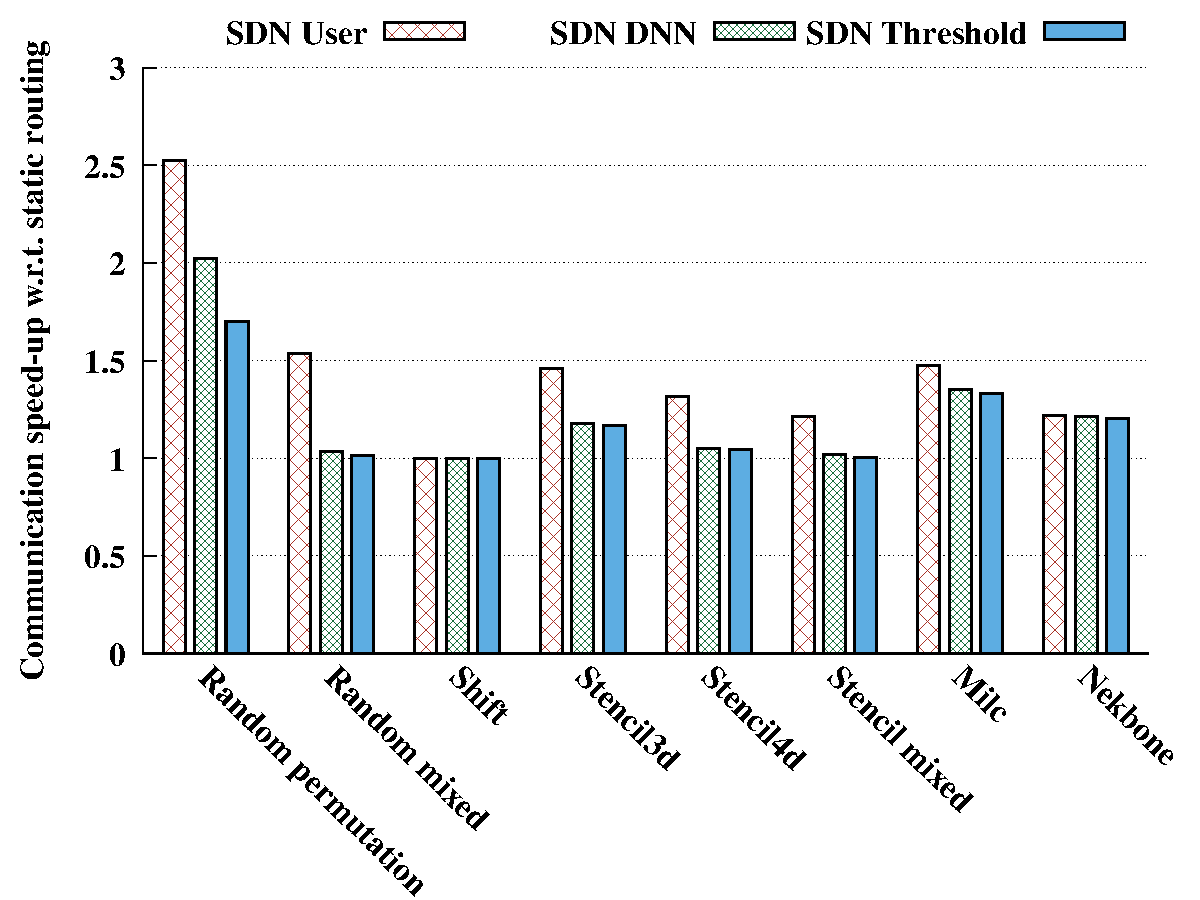
\includegraphics[width=\columnwidth]{./figs_4/full_fat_flow_detection.pdf}
  \caption{Comparison of flow detection in full bisection fat-tree of 1024 nodes}
  \label{fig:fld_full}
\end{figure}

Figure ~\ref{fig:fld_full} presents the communication speed-ups I obtained with three flow-identification strategies, SDN User, SDN DNN, and SDN Threshold—relative to a static routing baseline. Any bar exceeding unity indicates that my method reduced communication time with respect to static routing. Across every workload, I observe that the SDN User scheme delivers the greatest acceleration because it tags elephant flows at their inception and reroutes them accordingly from the start of the simulation. In the random permutation kernel, for example, SDN User achieves a 2.52× speed-up, whereas SDN DNN and SDN Threshold reach only 2.02× and 1.69×, respectively. The same pattern holds for production codes: my SDN User configuration accelerates stencil 4d by 1.32×, MILC by 1.48×, and Nekbone by 1.22×, each time outperforming the threshold detector. SDN DNN consistently ranks second. Although it incurs a fixed 0.3 ms classification latency, I find that its data-driven model recognises the repetitive communication patterns of HPC applications more rapidly than the polling-based threshold approach. This advantage is most evident in random permutation, with more than a 20 percent improvement over the threshold method, and it persists in real applications such as Nekbone, where SDN DNN attains a speed-up of 1.40 compared with 1.30 for the traditional threshold-based detector.Taken collectively, my results indicate that augmenting SDN routing with user-phase detection and a lightweight DNN classifier confers a statistically significant performance advantage over static routing. Moreover, this hybrid scheme matches or exceeds the communication efficiency of the conventional threshold-based detector while achieving faster flow-classification latency.

\subsubsection{Performance under 3-to-1 tapered fat-tree}
\begin{figure}[h]
  \centering
  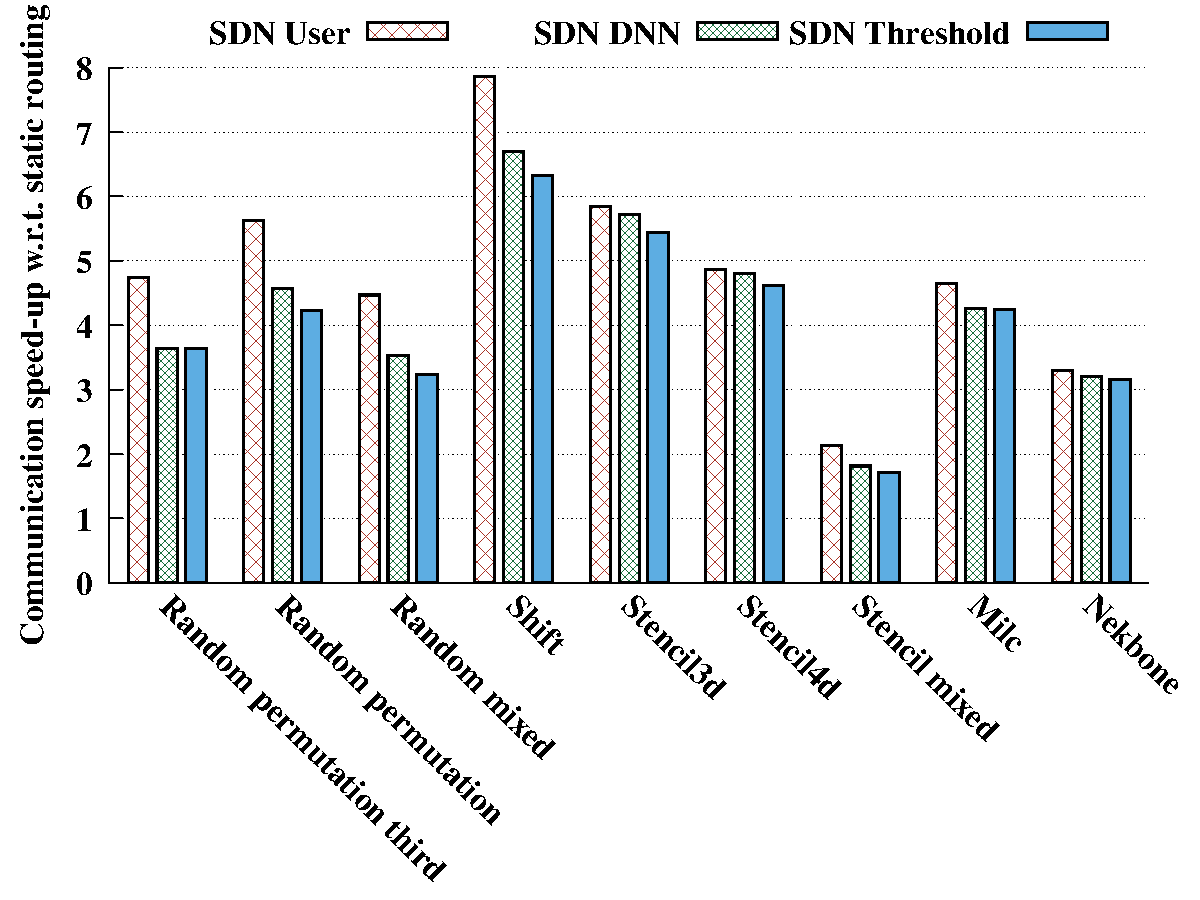
\includegraphics[width=\columnwidth]{./figs_4/taper_fat_flow_detection.pdf}
  \caption{Comparison of flow detection in 3 to 1 taper fat-tree of 1536 nodes}
  \label{fig:fld_taper}
\end{figure}

The Figure ~\ref{fig:fld_taper} illustrates the communication speedup achieved by different flow detection techniques (SDN User, SDN DNN, and SDN Threshold) under a 3-to-1 taper fat-tree topology with 1536 nodes and a 3:1 tapering ratio. This topology emphasizes the impact of reduced bandwidth at higher levels of the fat-tree structure. In a 3-to-1 tapered fat-tree topology, even a random permutation pattern represents a relatively dense communication workload. To better demonstrate the effectiveness of my technique, I introduced Random permutation third by removing two-thirds of the communication from a random permutation of 1536 nodes, retaining only eight out of the 24 communication flows passing through a leaf router. My evaluation revealed that SDN User consistently achieved the highest speedup, on an average 4 times faster compared to static routing, highlighting the benefits of early user-provided flow identification that enables optimal traffic balancing from the start. In contrast, SDN DNN and SDN Threshold exhibited moderate speedups of approximately 1.5x and 1.2x, respectively, due to delayed flow detection. In real applications such as Milc and Nekbone, the performance gap between techniques narrowed, though SDN User remained the top performer. 

\subsection{Evaluation of Phase Identification}
This section examines how different phase-identification schemes perform across multiple applications on both a full-bisection fat-tree and a 3-to-1 tapered fat-tree. Throughout the tests I fixed routing to SDN-optimal and activated the SDN-user flow detector, changing only the phase-identification method.
\subsubsection{Performance under full bisection fat-tree}


\begin{figure}[h]
  \centering
  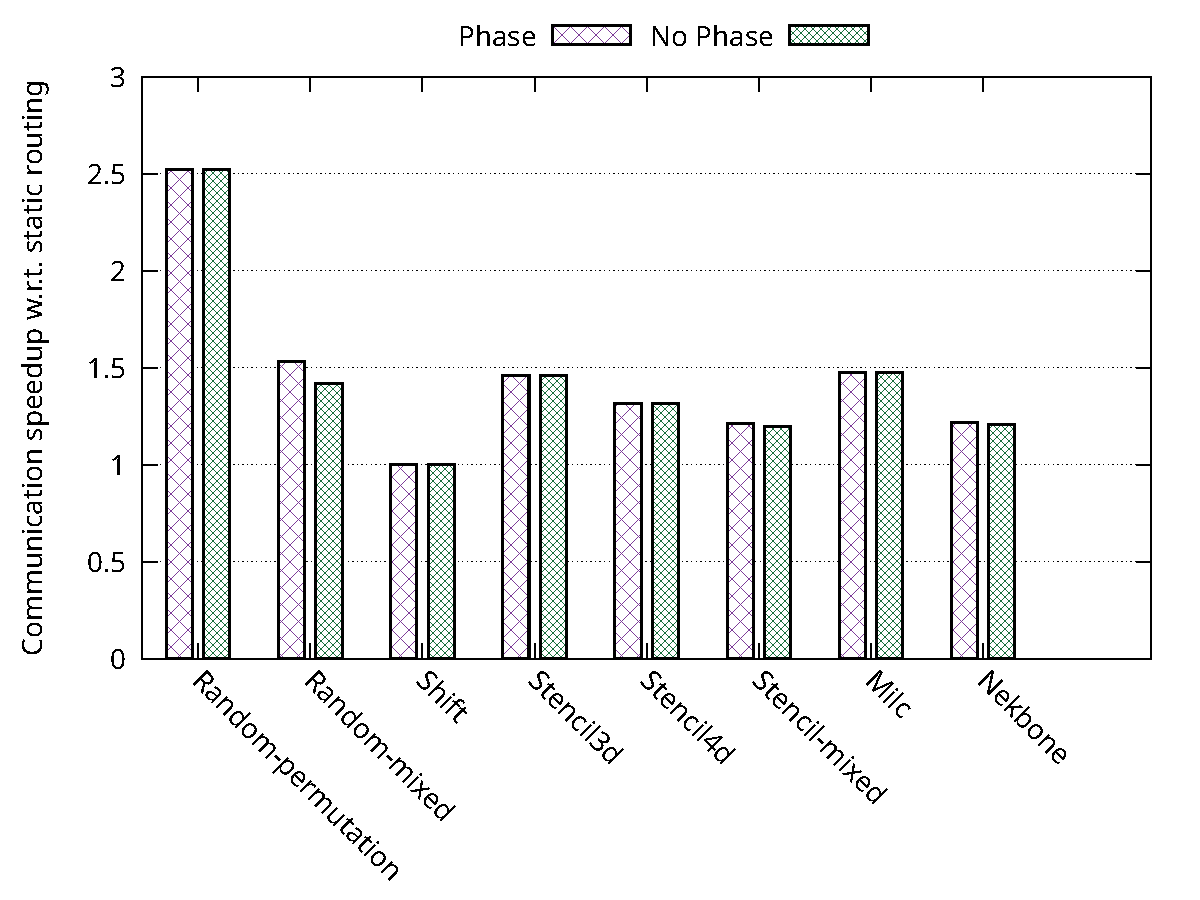
\includegraphics[width=\columnwidth]{./figs_4/phase_full.pdf}
  \caption{Comparison of phase identification in full bisection fat-tree of 1024 nodes}
  \label{fig:phase_full}
\end{figure}
Figure \ref{fig:phase_full} presents the communication speed-ups I obtained with three phase-identification strategies, User-phase, Dynamic-phase, and No-phase, relative to a static-routing baseline. 
Any bar exceeding unity indicates that phase awareness allowed the network to shorten communication time. 
I focus on the random mixed and stencil mixed kernels, where I deliberately inserted computation intervals to expose the benefits of phase detection. Across both workloads the User-phase scheme delivers the largest acceleration, because the application signals each phase boundary and the controller can release bandwidth immediately. 
In random mixed, User-phase attains a 1.53× speed-up, whereas Dynamic-phase and No-phase reach only 1.48× and 1.40×, respectively. A similar pattern emerges in stencil-mixed where the User-phase achieves 1.21×, Dynamic-phase 1.20×, and No-phase 1.11×. Dynamic-phase consistently ranks second as it has a delay of 100ms to detect a phase change. Although it incurs that delay, its on-line inference still recognises the shift from communication to computation which helps is releasing the resources quickly. 

\subsubsection{Performance under 3-to-1 tapered fat-tree}
Figure \ref{fig:phase_taper} presents the communication speed-ups with different phase identification techniques in 1536-node, 3-to-1 tapered fat-tree. Here, in random-mixed, User-phase achieves a 4.53× speed-up, whereas dynamic-phase and no-phase reach 4.42× and 4.18×, respectively; thus, explicit phase cues deliver an additional 8\% benefit over dynamic phase detector that waits for 100 ms to infer phase changes. A similar pattern appears in stencil-mixed, where user-phase attains 2.21×, dynamic-phase 2.15×, and no-phase 2.04×. 

\begin{figure}[h]
  \centering
  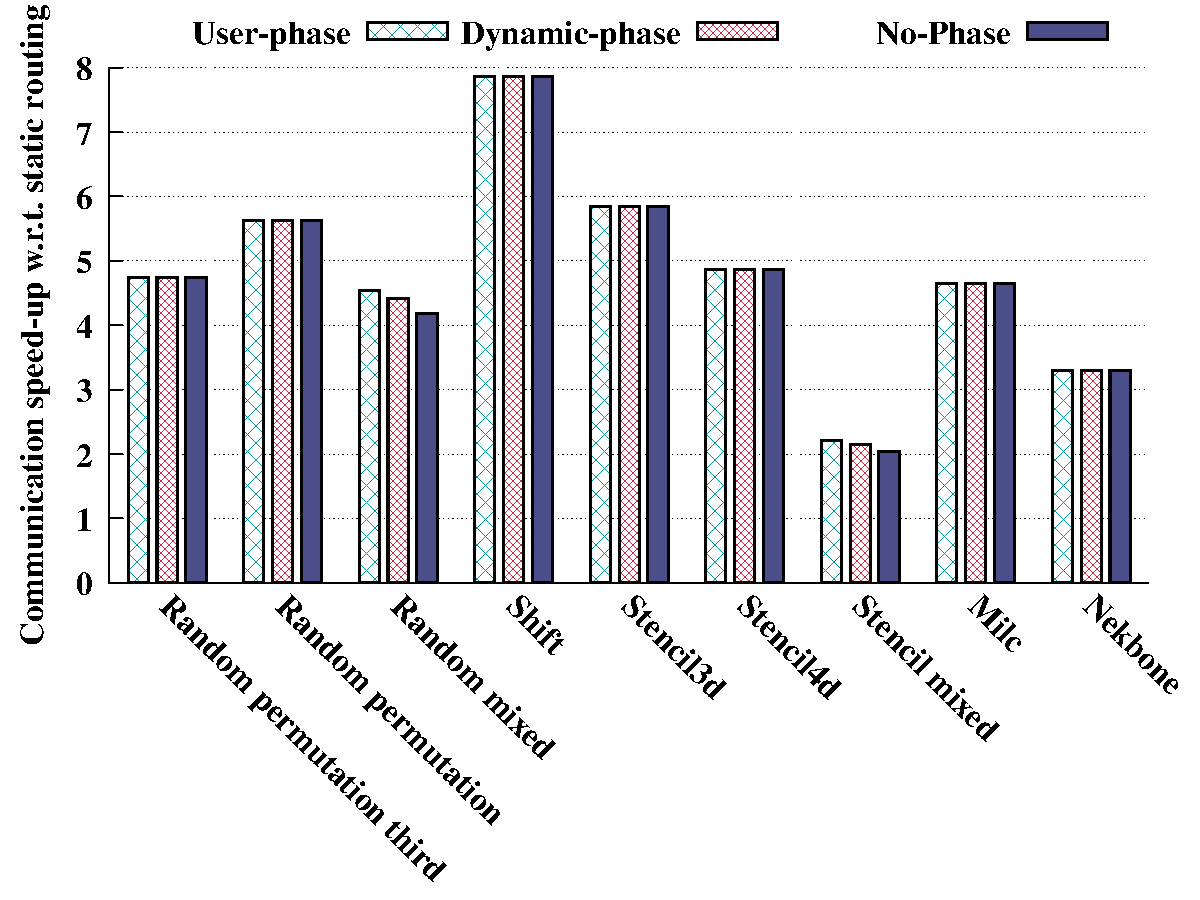
\includegraphics[width=\columnwidth]{./figs_4/phase_taper.pdf}
  \caption{Comparison of phase identification in full bisection fat-tree of 1536 nodes}
  \label{fig:phase_taper}
\end{figure}


Taken together, these data indicate that phase-based optimisation combined with SDN routing is especially valuable in fat-tree topologies, where user supplied phase information yields the greatest benefit, a lightweight DNN detector closes most of the gap while avoiding additional efforts from user to pre-determine the phases, and both approaches outperform the case where no phase detection is performed.

\subsection{Evaluation of SDN-based Routing}
In this section, I assess the efficacy of several SDN routing strategies over two network topologies, a full-bisection fat-tree and a 3-to-1 tapered fat-tree. To isolate the influence of the routing algorithm, I keep the phase identification scheme as User-phase and the flow detection scheme as SDN User, varying only the routing method itself across the experiments.

\subsubsection{Performance under full bisection fat-tree}
Figure \ref{fig:routing_full} makes clear that software-defined routing delivers
a substantial and consistent benefit over static routing. All three SDN routing
schemes, SDN-greedy, SDN-optimal, and SDN-adaptive has a communication speed-up well above 1, meaning they
always shorten application communication time compared to single path static routing without SDN features. The effect is most pronounced in the
random permutation workload, where SDN-optimal reaches a 2.52×
speed-up (a 152 % reduction in time), because here a link is used by only one flow, as a result there is no contention in the whole network. Even the lightweight SDN-greedy records
2.10× speed-up in random permutation. Real applications like Milc and Nekbone shows the same pattern. In the four-dimensional stencil4d
kernel SDN-optimal achieves 1.32×, and in the computation-heavy MILC
application it still provides a 1.48× gain. These results indicate that simply
enabling an SDN controller so that every path is chosen centrally and made
contention-free can more than double communication
performance.
Adaptive multipath routing, the current state-of-the-art multipath alternative,
occasionally edges ahead of SDN in very dense traffic (for example, a 1.97×
boost in MILC), yet it also falls below the static baseline in the shift
benchmark, where a single permutation when made to share paths leads to some congestion. For this kind of situations where the traffic density is low or moderate, a hybrid SDN-adaptive mode recovers that loss by defaulting to the
optimal SDN paths at start-up. Taken together, the data shows that SDN routing
consistently surpasses static routing and in many cases exceeds
adaptive routing, establishing centralized, contention-free path selection as a powerful
and practical tool for accelerating HPC communication.

\begin{figure}[h]
  \centering
  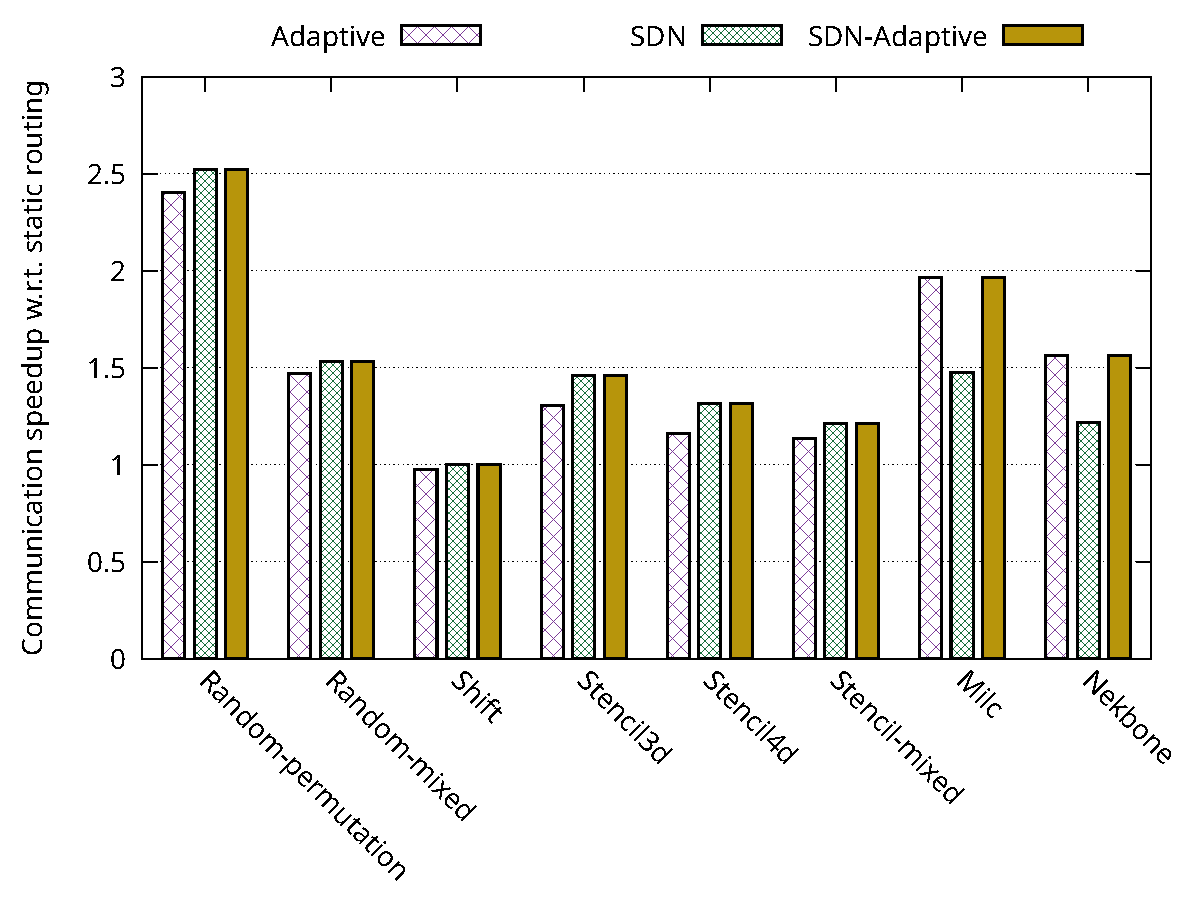
\includegraphics[width=\columnwidth]{./figs_4/routing_full.pdf}
  \caption{Comparison of routing techniques in full fat-tree of 1024 nodes}
  \label{fig:routing_full}
\end{figure}

\subsubsection{Performance under 3-to-1 tapered fat-tree}
Figure \ref{fig:routing_taper} makes clear that SDN routing gives very large gains over static routing on the 1536-node, 3-to-1 tapered fat-tree. The SDN-optimal scheme is best overall, cutting communication time by factors of 7.87× in shift, 5.63× in random permutation, and 4.75× in random permutation third. Even the simpler SDN-greedy still reaches 5.31×, 4.21×, and 4.12× in the same three workloads. 
Tapering removes two-thirds of the upward bandwidth, so a full random permutation already counts as a moderately dense workload: many flows share the same core links, and multipath adaptive can spread them slightly better than single-path SDN-optimal (5.74× versus 5.63×). When I thin the traffic to random-permutation-third, each core link carries only one flow; under this simpler pattern SDN-optimal’s centrally chosen, contention-free paths move ahead of adaptive (4.75× versus 4.60×). The same reversal appears in shift (7.87× versus 7.63×). In the very dense Milc and stencil3d kernels, however, adaptive keeps a small lead because its many paths can still distribute heavy load more evenly.
In summary, all SDN variants improve communication speed-up by roughly four- to eight-fold compared with static routing, and the hybrid SDN-adaptive mode matches SDN-optimal or adaptive routing in every case by switching to the globally computed paths or adaptive routing at start-up. These results show that, in a tapered fat-tree where congestion is stronger, centrally coordinated SDN routing can work better than the traditional static or adaptive routing widely used in fat-tree interconnect based HPC systems.
\begin{figure}[h]
  \centering
  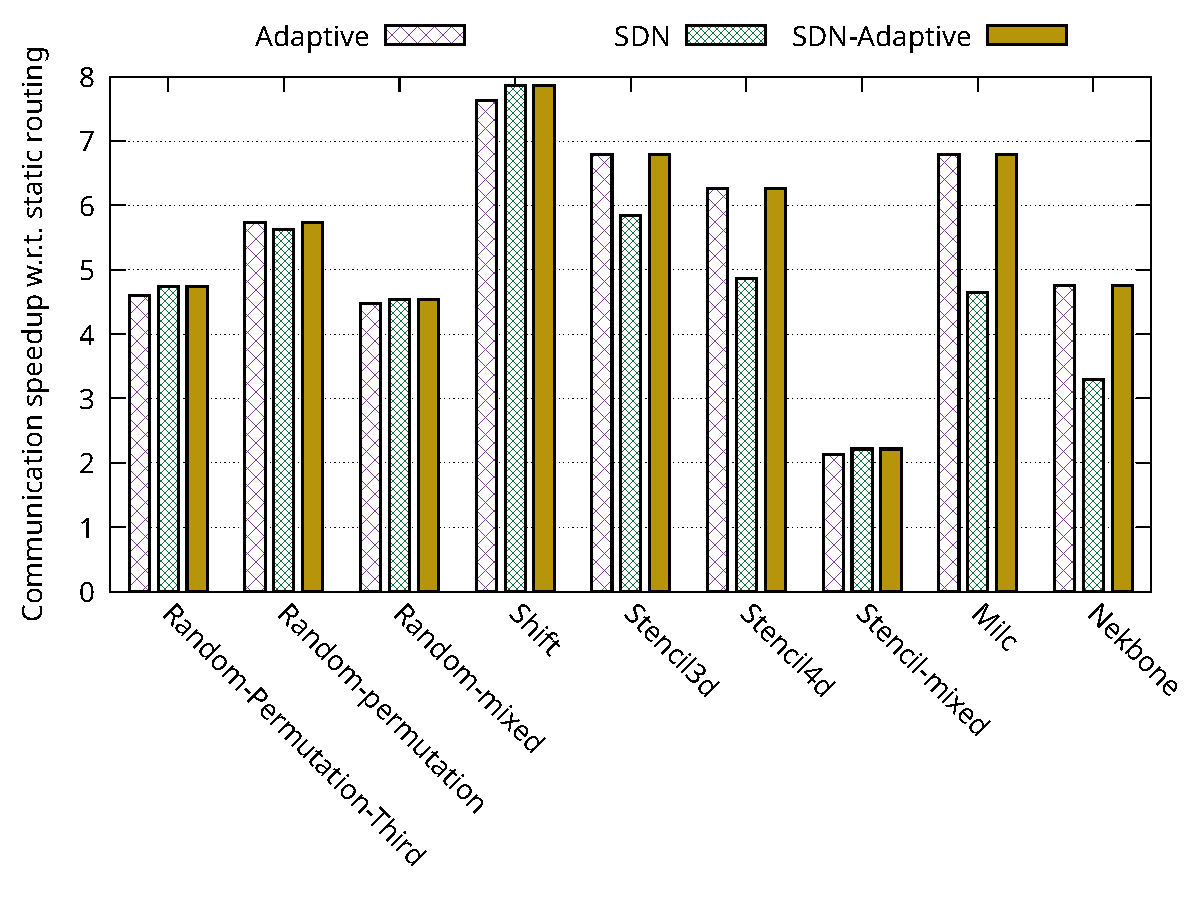
\includegraphics[width=\columnwidth]{./figs_4/routing_taper.pdf}
  \caption{Comparison of routing techniques in 3 to 1 taper fat-tree of 1536 nodes}
  \label{fig:routing_taper}
\end{figure}
